% Generated by LitigCharts.PublicationFigures. Captions and provenance are sidecars.
\documentclass[10pt,tikz,border=5pt]{standalone}
\usepackage{lmodern}
\usetikzlibrary{patterns,patterns.meta}
\begin{document}
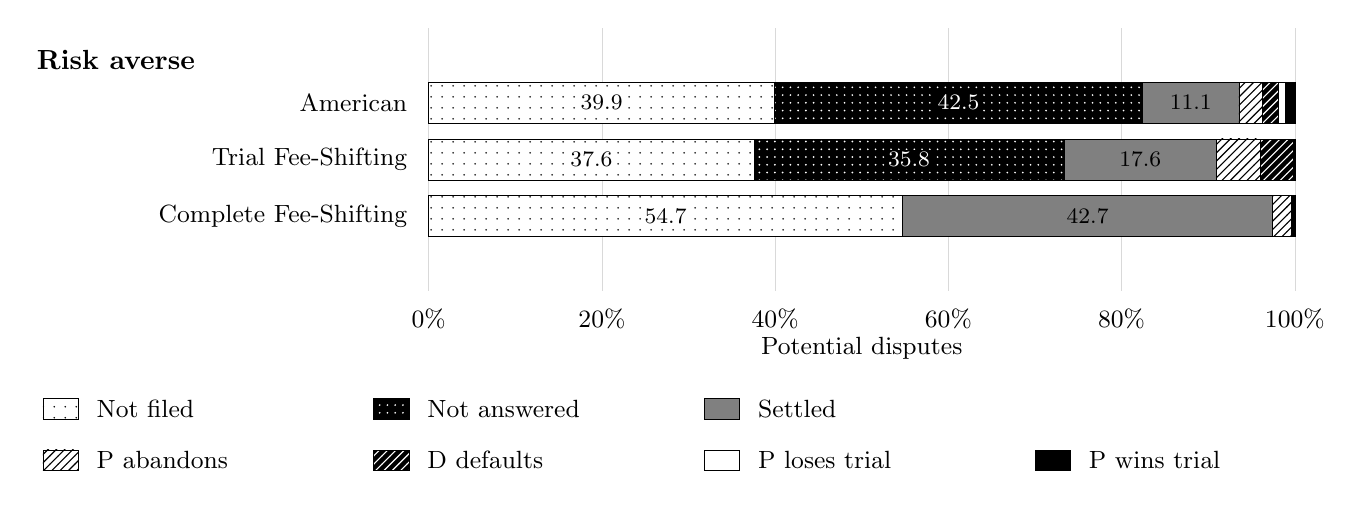
\begin{tikzpicture}[font=\small]\draw[black!15,line width=.2pt] (5.1,.65) -- (5.1,3.99);
\node[anchor=north] at (5.1,.55) {0\%};
\draw[black!15,line width=.2pt] (7.3,.65) -- (7.3,3.99);
\node[anchor=north] at (7.3,.55) {20\%};
\draw[black!15,line width=.2pt] (9.5,.65) -- (9.5,3.99);
\node[anchor=north] at (9.5,.55) {40\%};
\draw[black!15,line width=.2pt] (11.7,.65) -- (11.7,3.99);
\node[anchor=north] at (11.7,.55) {60\%};
\draw[black!15,line width=.2pt] (13.9,.65) -- (13.9,3.99);
\node[anchor=north] at (13.9,.55) {80\%};
\draw[black!15,line width=.2pt] (16.1,.65) -- (16.1,3.99);
\node[anchor=north] at (16.1,.55) {100\%};
\node[anchor=west,font=\bfseries] at (0,3.59) {\mbox{Risk} \mbox{averse}};
\node[anchor=east] at (4.95,3.04) {American};
\path[preaction={fill=white,draw=none},pattern={Dots[distance=4pt,radius=.35pt]},pattern color=black,draw=black,line width=.25pt] (5.1,2.78) rectangle (9.49186,3.3);
\node[text=black,fill=white,font=\footnotesize,inner sep=1pt] at (7.29593,3.04) {39.9};
\path[preaction={fill=black,draw=none},pattern={Dots[distance=2.8pt,radius=.35pt]},pattern color=white,draw=black,line width=.25pt] (9.49186,2.78) rectangle (14.165947,3.3);
\node[text=white,fill=black,font=\footnotesize,inner sep=1pt] at (11.828904,3.04) {42.5};
\path[fill=black!50,draw=black,line width=.25pt] (14.165947,2.78) rectangle (15.389719,3.3);
\node[text=black,fill=none,font=\footnotesize,inner sep=1pt] at (14.777833,3.04) {11.1};
\path[preaction={fill=white,draw=none},pattern={north east lines},pattern color=black,draw=black,line width=.25pt] (15.389719,2.78) rectangle (15.686424,3.3);
\path[preaction={fill=black,draw=none},pattern={north east lines},pattern color=white,draw=black,line width=.25pt] (15.686424,2.78) rectangle (15.889747,3.3);
\path[fill=white,draw=black,line width=.25pt] (15.889747,2.78) rectangle (15.977294,3.3);
\path[fill=black,draw=black,line width=.25pt] (15.977294,2.78) rectangle (16.099994,3.3);
\node[anchor=east] at (4.95,2.32) {Trial Fee-Shifting};
\path[preaction={fill=white,draw=none},pattern={Dots[distance=4pt,radius=.35pt]},pattern color=black,draw=black,line width=.25pt] (5.1,2.06) rectangle (9.232975,2.58);
\node[text=black,fill=white,font=\footnotesize,inner sep=1pt] at (7.166488,2.32) {37.6};
\path[preaction={fill=black,draw=none},pattern={Dots[distance=2.8pt,radius=.35pt]},pattern color=white,draw=black,line width=.25pt] (9.232975,2.06) rectangle (13.167345,2.58);
\node[text=white,fill=black,font=\footnotesize,inner sep=1pt] at (11.20016,2.32) {35.8};
\path[fill=black!50,draw=black,line width=.25pt] (13.167345,2.06) rectangle (15.105171,2.58);
\node[text=black,fill=none,font=\footnotesize,inner sep=1pt] at (14.136258,2.32) {17.6};
\path[preaction={fill=white,draw=none},pattern={north east lines},pattern color=black,draw=black,line width=.25pt] (15.105171,2.06) rectangle (15.663753,2.58);
\path[preaction={fill=black,draw=none},pattern={north east lines},pattern color=white,draw=black,line width=.25pt] (15.663753,2.06) rectangle (16.077568,2.58);
\path[fill=white,draw=black,line width=.25pt] (16.077568,2.06) rectangle (16.087933,2.58);
\path[fill=black,draw=black,line width=.25pt] (16.087933,2.06) rectangle (16.100002,2.58);
\node[anchor=east] at (4.95,1.6) {Complete Fee-Shifting};
\path[preaction={fill=white,draw=none},pattern={Dots[distance=4pt,radius=.35pt]},pattern color=black,draw=black,line width=.25pt] (5.1,1.34) rectangle (11.117594,1.86);
\node[text=black,fill=white,font=\footnotesize,inner sep=1pt] at (8.108797,1.6) {54.7};
\path[fill=black!50,draw=black,line width=.25pt] (11.117594,1.34) rectangle (15.818686,1.86);
\node[text=black,fill=none,font=\footnotesize,inner sep=1pt] at (13.46814,1.6) {42.7};
\path[preaction={fill=white,draw=none},pattern={north east lines},pattern color=black,draw=black,line width=.25pt] (15.818686,1.34) rectangle (16.053248,1.86);
\path[fill=white,draw=black,line width=.25pt] (16.053248,1.34) rectangle (16.064628,1.86);
\path[fill=black,draw=black,line width=.25pt] (16.064628,1.34) rectangle (16.099999,1.86);
\node at (10.6,-.08) {Potential disputes};
\path[preaction={fill=white,draw=none},pattern={Dots[distance=4pt,radius=.35pt]},pattern color=black,draw=black,line width=.25pt] (0.2,-0.98) rectangle (0.65,-0.72);
\node[anchor=west] at (0.76,-0.85) {Not filed};
\path[preaction={fill=black,draw=none},pattern={Dots[distance=2.8pt,radius=.35pt]},pattern color=white,draw=black,line width=.25pt] (4.4,-0.98) rectangle (4.85,-0.72);
\node[anchor=west] at (4.96,-0.85) {Not answered};
\path[fill=black!50,draw=black,line width=.25pt] (8.6,-0.98) rectangle (9.05,-0.72);
\node[anchor=west] at (9.16,-0.85) {Settled};
\path[preaction={fill=white,draw=none},pattern={north east lines},pattern color=black,draw=black,line width=.25pt] (0.2,-1.63) rectangle (0.65,-1.37);
\node[anchor=west] at (0.76,-1.5) {P abandons};
\path[preaction={fill=black,draw=none},pattern={north east lines},pattern color=white,draw=black,line width=.25pt] (4.4,-1.63) rectangle (4.85,-1.37);
\node[anchor=west] at (4.96,-1.5) {D defaults};
\path[fill=white,draw=black,line width=.25pt] (8.6,-1.63) rectangle (9.05,-1.37);
\node[anchor=west] at (9.16,-1.5) {P loses trial};
\path[fill=black,draw=black,line width=.25pt] (12.8,-1.63) rectangle (13.25,-1.37);
\node[anchor=west] at (13.36,-1.5) {P wins trial};
\end{tikzpicture}
\end{document}
